\documentclass[10pt,A4,makeidx]{article}
\usepackage{graphicx}
\usepackage{grffile}
\usepackage{color}
\usepackage{amsmath}
\usepackage{float}
\usepackage{subfig}
\usepackage{comment}
\UseRawInputEncoding

\graphicspath{ {./visuals/} }

\textwidth 16.5cm
\hoffset -2.0cm
\textheight 24cm
\voffset -2.5cm

\newcommand{\tR}{\texttt{R}}
\newcommand{\adist}{\overset{\cdot}{\underset{\cdot}{\sim}}}
%\setcounter{tocdepth}{2}

\title
{Effects of Structural Characteristics on House Prices}
\author{Sean Peralta Garcia (23088091)}
\date {}

\usepackage{Sweave}
\begin{document}

\maketitle


\section{Executive Summary}
\section{Introduction}
  Owning a house is one of the biggest investments a person can make. As such, it 
  is of great interest to prospective buyers, sellers and lenders to accurately
  predict the price of a home. There are a range of models and techniques that 
  attempt to predict the price of a home, from observational appraisals all 
  the way to machine learning models[2]. One method widely studied is that of
  hedonic pricing. A Hedonic Pricing Model (henceforth, HPM) is a model that 
  attempts to estimate the price of a good by taking its observable characteristics
  and then weighting them according to their relative impact on the price. Models
  utilise a range of measures that can be categorised into several groups, 
  namely structural, neighbourhood, and environmental.[3] Hearth and Maier,
  in a literature review of HPMs for real estate, had identified that the 
  neighbourhood and environmental factors were generally over-researched. While
  social factors and the "implicit value of structural characteristics" was 
  under-researched.[1]

  \subsection{Related Work}
  There appears to be a consensus that creating a HPM, particularly focussing on
  structural characteristics, has problems with heteroskedasticity. This means
  that linear models may not be entirely appropriate to estimate the response.
  This was sought to be relieved by Selim, Limsombunchai and Malpezzi by using
  a semi-logarithmic form wherein the response variable is transformed by the natural log.[2, 3, 4]
  Additionally, Malpezzi explains
  that this effectively allows value added to the house to be proportional to 
  other variables in the model and for an easier interpretation of coefficients
  such that the coefficient of a measure is the percentage change for 1 unit 
  difference in the measure.[3]
  In the end Selim concluded that water system, presence of a pool, the type of house,
  number of rooms, house size, locational characteristics and building type were
  the most significant variables to affect house prices in the country of Turkey.[4]
    
  \subsection{Data Set}
  The data set contains data on houses in Saratoga County, New York; collected by
  Candice Corvetti in 2006. It contains 1063 randomly selected observations collecting
  data on house price, size in square feet, number of bathrooms, number of bedrooms,
  the presence of a fireplace, land size in acres and the age of the house in years.
  
  \subsection{Aim}
  The aim of this report is to fit a model that will attempt to determine how 
  the price of a house depends its structural characteristics. Significant 
  variables that appear in the Turkish model will be explored in the Saratoga 
  data set to see if they also play a significant role in predicting house price.

\section{Methodology}
The methodology to be used in this report will be split into two parts. Data
exploration and model fitting.
  \subsection{Data Exploration}
  Firstly, the scatter plots between independent and dependent variables will be 
  visually analysed to identify relationships and distribution of data. Strangely
  distributed data will attemp to be transformed to find a linear relationship to 
  the price. After, scatter plots between independent variables will be visually analysed to quickly 
  identify multicollinear variables. Additionally, correlation analysis will be used to 
  supplement the visual analyses. This process will aim to identify redundant and 
  non-contributing variables that we can safely assume can be excluded from the 
  final model.  
  Variables that are suspected to have interaction are investigated by running linear 
  regressions with only those interaction terms and analysing the interaction plots.
  If an interaction effect is apparent then that interaction term will be considered
  in model fitting.
  \subsection{Model fitting}
  Model fitting will be done with backwards elimination, including found interaction 
  variables. Firstly, the collinear variables will be removed from the model and 
  tested using the F-test to check for a better fit. Then normal backwards elimination 
  will be applied.
\section{Results}
  \subsection{Data Exploration}

  Below are the relationships between the Price and independent variables.\\
  \emph{Correlation data in appendix figure 1 and 2.}
  \begin{itemize}
    \item Size - exhibits a strong, positive linear relationship. (correlation: 0.77)
    \item Baths - exhibits a moderate, positive linear relationship. (correlation: 0.67)
    \item Bedrooms - exhibits a weak linear relationship (correlation: 0.47)
    \item Fireplace - exhibits a weak, positive linear relationship - houses 
    with a fireplace have a higher range of price, as well as a higher mean (correlation: 0.41)
    \\(\emph{Correlation data in appendix figure 3.})
    \item Acres - little to no linear relationship - data is heavily left skewed (\emph{see below})  
      \subitem - acres are all clustered closer to 0 (correlation: 0.18)
    \item Age - little to no linear relationship - heavily left skewed (\emph{see below})
      \subitem - majority of properties are grouped
    towards 0 age (correlation: -0.26)\\
  \end{itemize}
  
  Due to the low correlations of fireplace, acres and age, we can assume that
  they are unlikely to come up in the final model.
  
  \begin{center}
    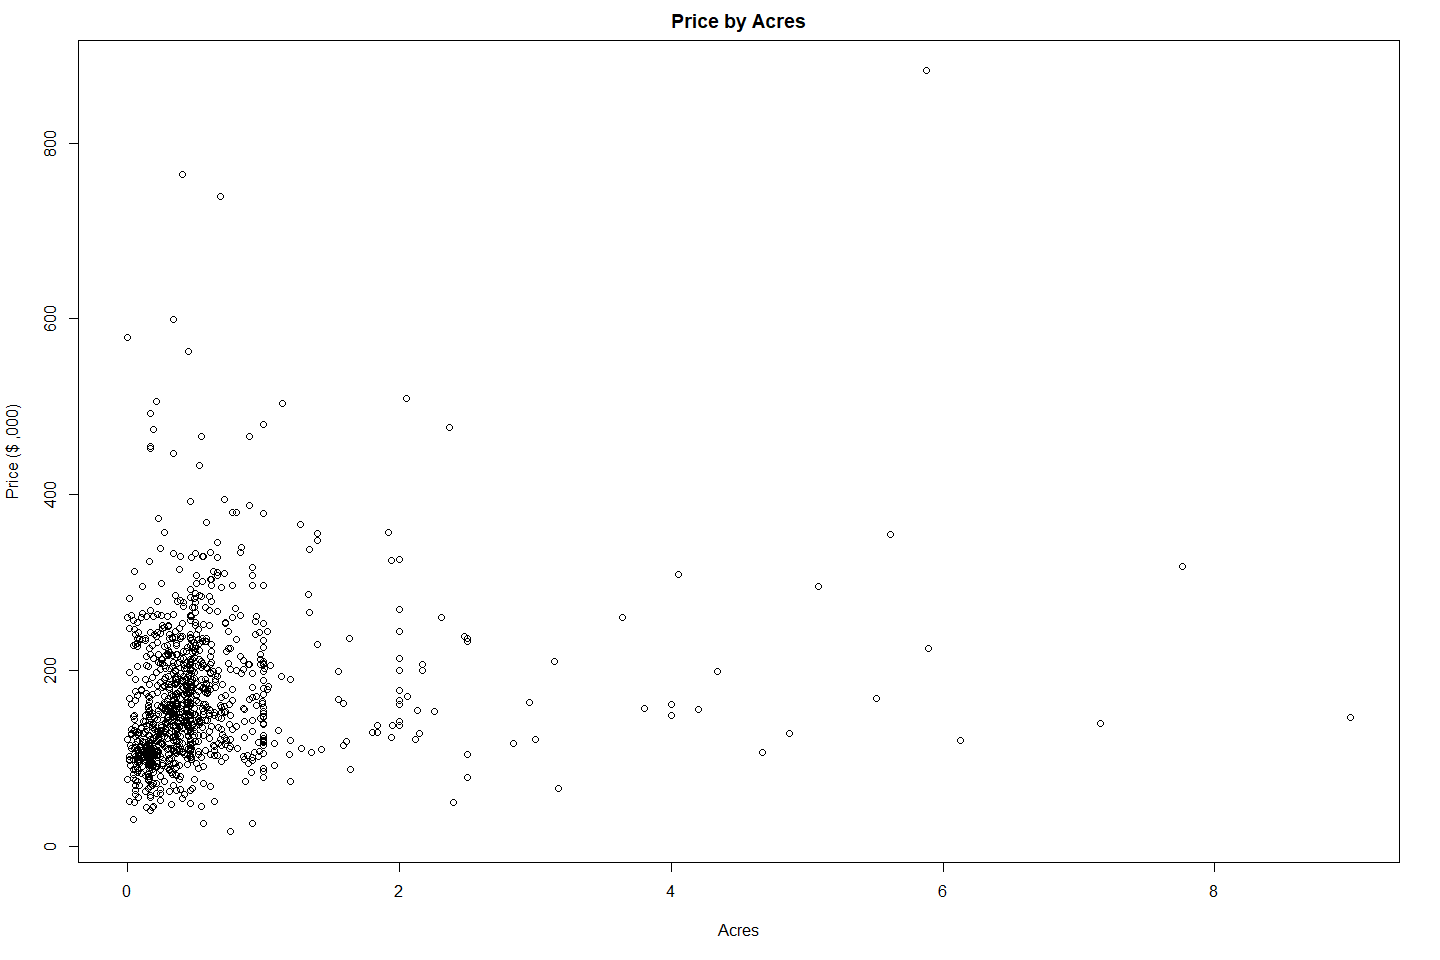
\includegraphics[width=8cm]{price-acres.png}
    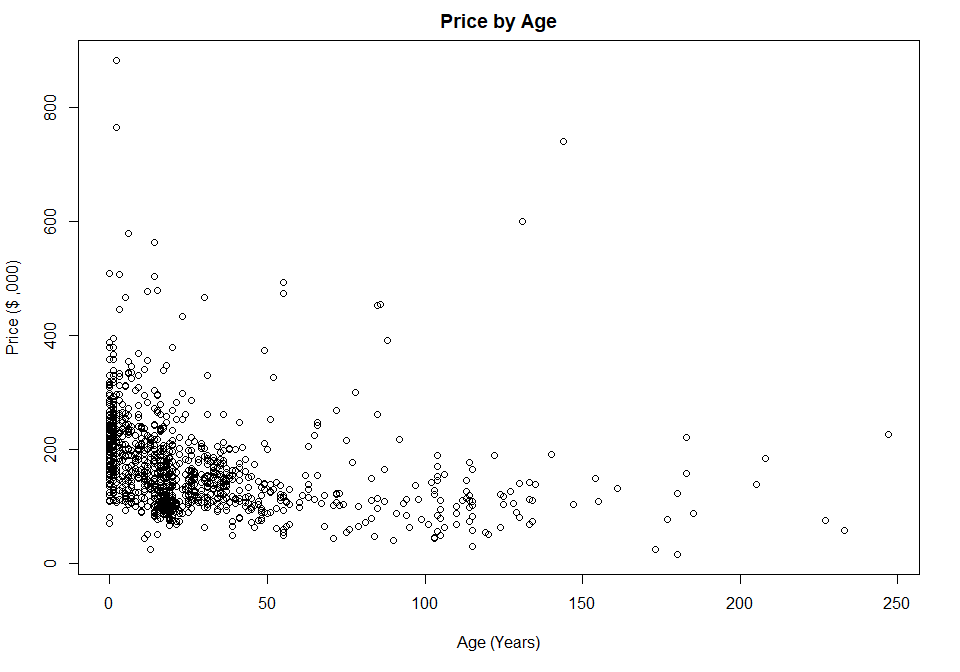
\includegraphics[width=8cm]{price-age.png}
  \end{center}
  
  Now we will find collinear variables by analysing 
  

  Now possible interaction terms will be investigated. The following are possible 
  interactions that will be investigated
  \begin{itemize}
  \item Baths:Size - some explanation
  \item Bedrooms:Size
  \item Acres:Size
  \item Fireplace:Age
  \end{itemize}

  \subsection{Model fitting}
  \begin{center}
    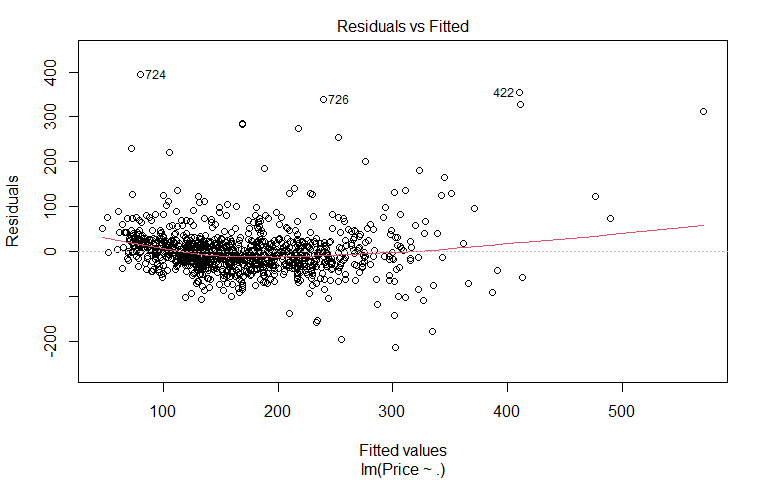
\includegraphics[width=8cm]{full-res.png}
    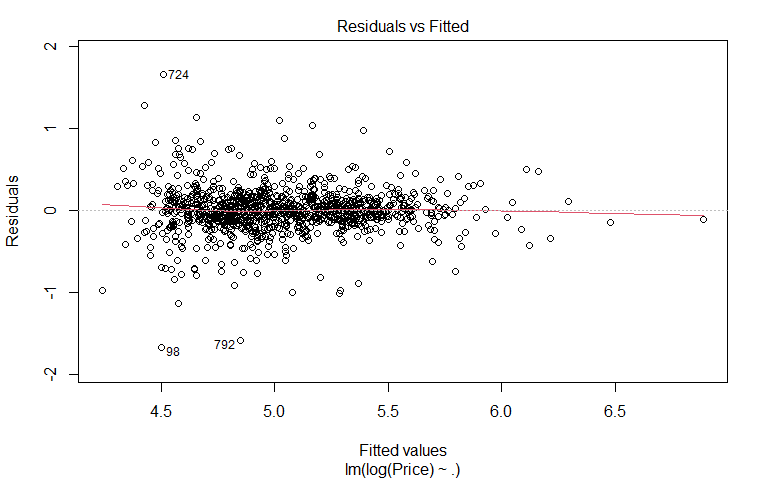
\includegraphics[width=8cm]{full-resln.png}
  \end{center}
  First fitted the full model - without interactions - to check residual plot
  (shows a non constant errors in residual plot) high RSE (52.15) - proof of 
  heteroskedasticity shown in the other studies.
  and then applied the  a natural log function to the reponse RSE as suggested by
  previous studies a lot - RSE lower (0.279) thus indicating a the response variable
  follows a log relationship to the independent variables in the model
\section{Discussion}
age and acres might have been able to be transformed in order to find a relationship

\bibliographystyle{apalike}
\begin{thebibliography}{9}
\bibitem{lit_rev}
Herath, S. K. Maier, G. (2010). The hedonic price method in real estate and housing market research. A review of the literature.. Institute for Regional Development and Environment (pp. 1-21). Vienna, Austria: University of Economics and Business.

\bibitem{hedonic_ai}
Limsombunchai, V. (2004). House price prediction: Hedonic price model vs. artificial neural network. New Zealand Agricultural and Resource Economics Society Conference, 25-26 June 2004. Blenheim, New Zealand: New Zealand Agricultural and Resource Economics Society.

\bibitem{hedonic_rev}
Malpezzi, S. (2003). Hedonic pricing models: a selective and applied review. Housing economics and public policy, 1, 67-89.

\bibitem{hedonic_regress}
Selim, S. (2008). DETERMINANTS OF HOUSE PRICES IN TURKEY: A HEDONIC REGRESSION MODEL . Dogus Universitesi Dergisi , 9 (1) , 65-76 . Retrieved from 
\end{thebibliography}

\pagebreak
\section*{Appendix.}
  \emph{\\Figure 1 - Correlation coefficients for untransformed data}
  \begin{Soutput}
              Price  Size Baths Bedrooms Fireplace Acres   Age
    Price      1.00  0.77  0.67     0.47      0.41  0.18 -0.26
    Size       0.77  1.00  0.74     0.67      0.47  0.22 -0.23
    Baths      0.67  0.74  1.00     0.51      0.45  0.13 -0.40
    Bedrooms   0.47  0.67  0.51     1.00      0.30  0.15 -0.04
    Fireplace  0.41  0.47  0.45     0.30      1.00  0.06 -0.24
    Acres      0.18  0.22  0.13     0.15      0.06  1.00  0.01
    Age       -0.26 -0.23 -0.40    -0.04     -0.24  0.01  1.00
  \end{Soutput}
  
  \emph{Figure 2 - All plots}\\
  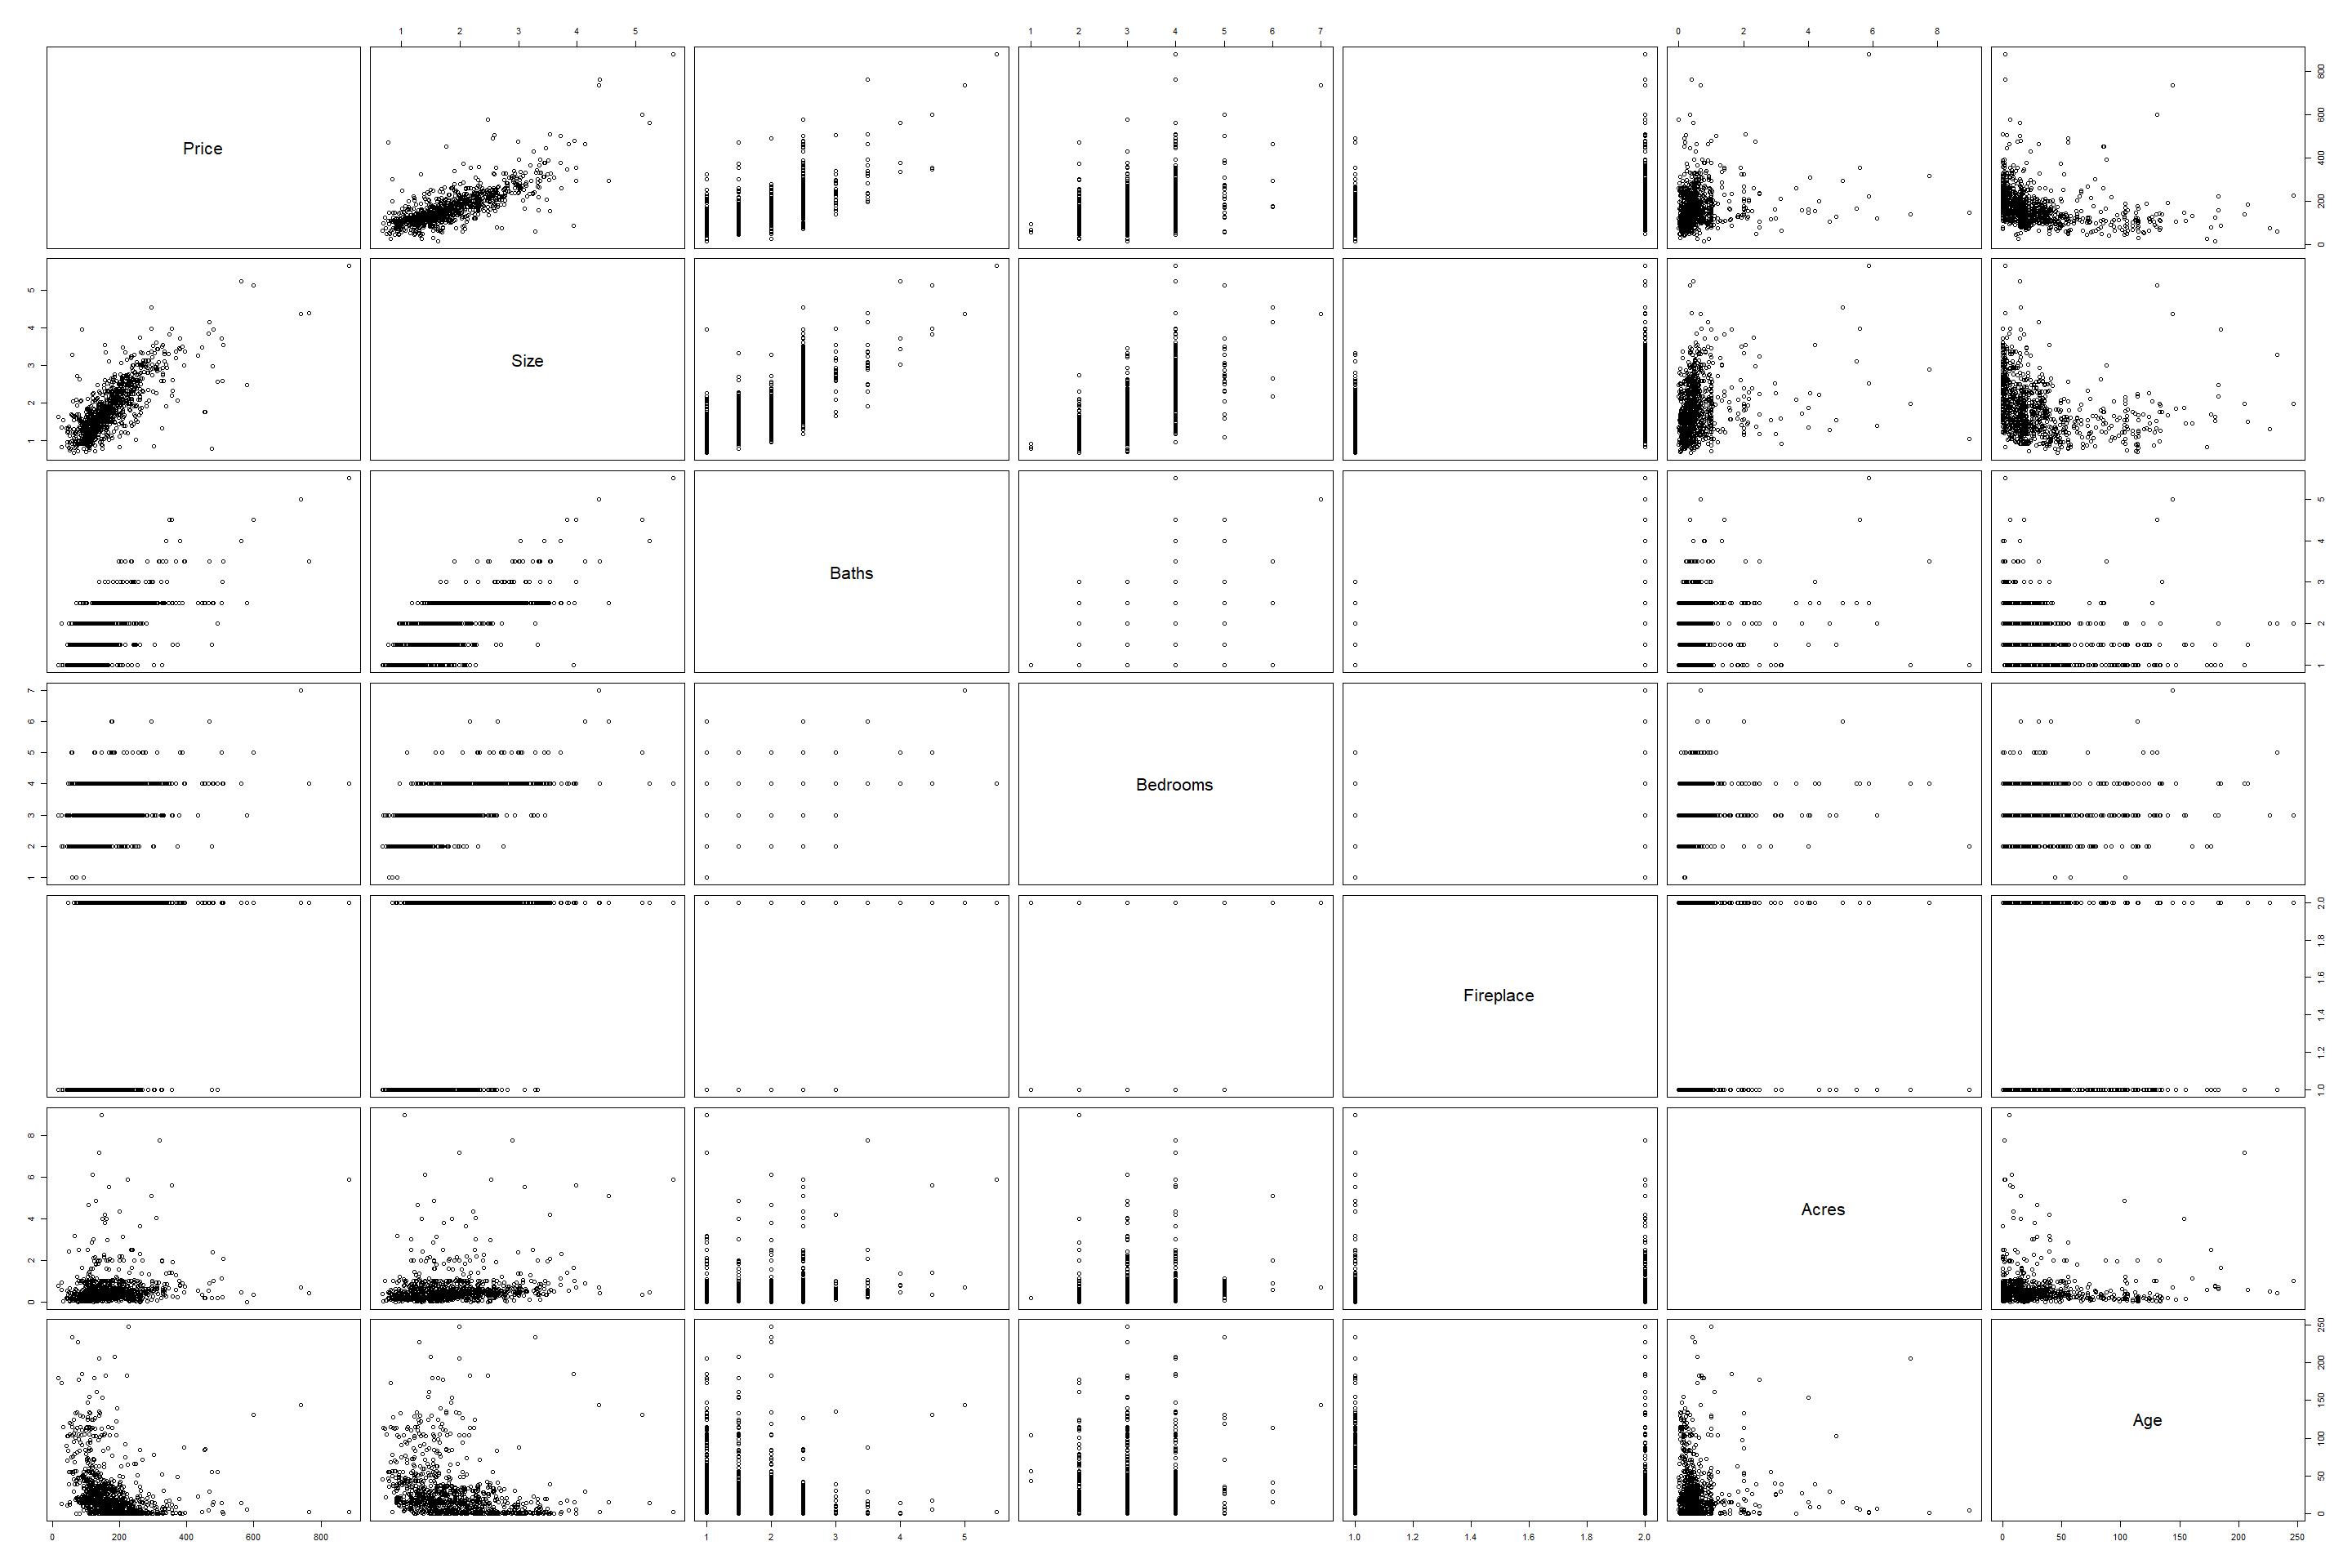
\includegraphics[scale=2]{plot.png}
  
  \emph{Figure 3 - Price by Fireplace boxplot}\\
  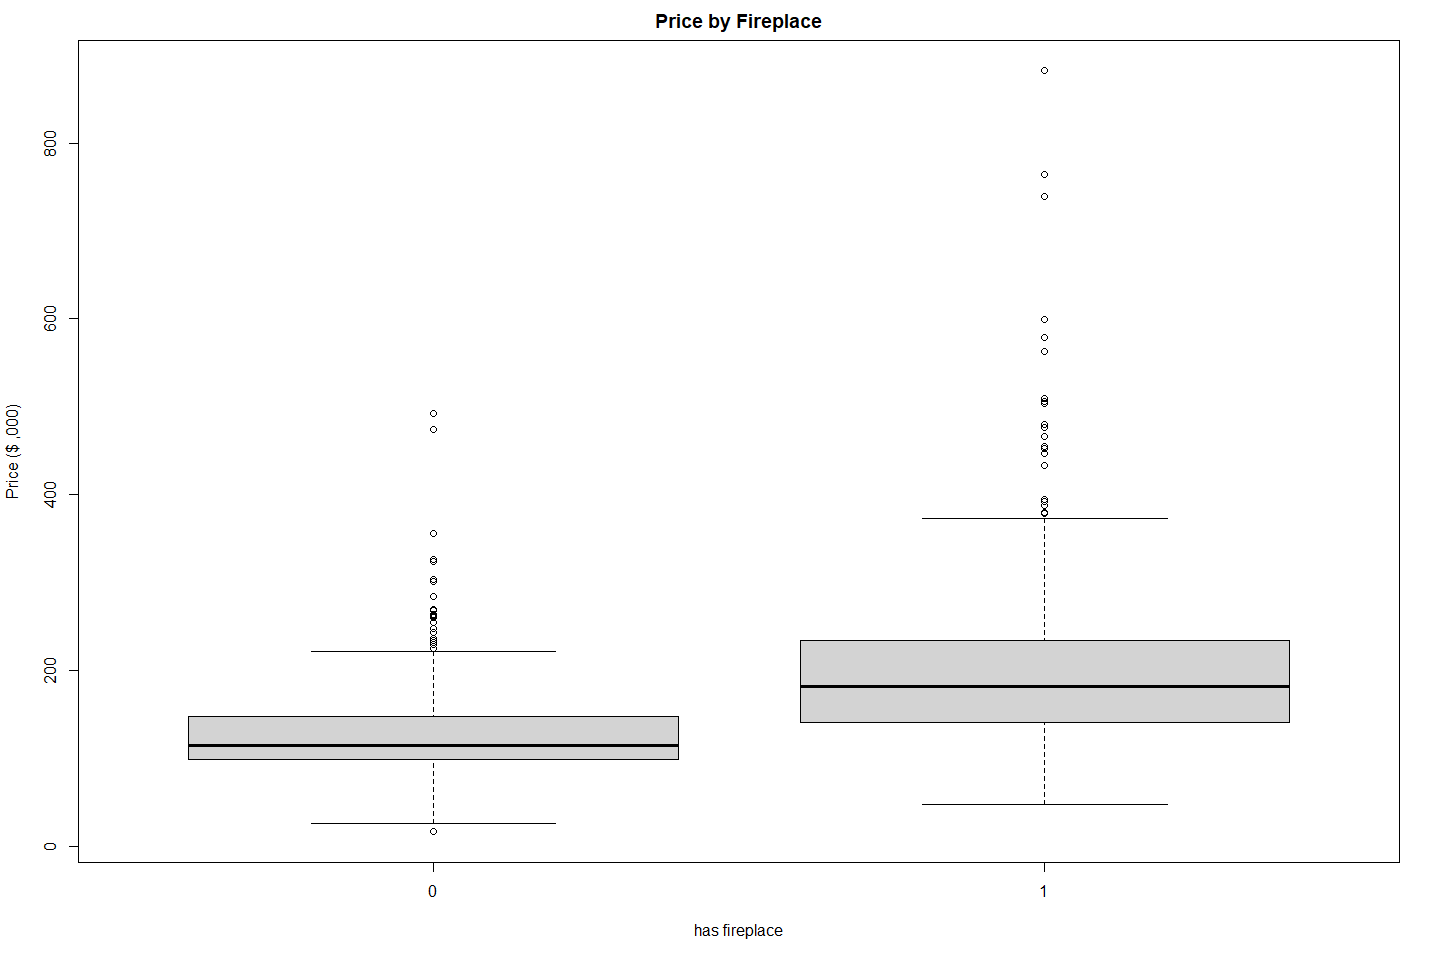
\includegraphics[scale=0.4]{price-fireplace.png}

\end{document}
